\chapter{Methods}
\extrafloats{100}
\maxdeadcycles=200

\section{The data}
PLease tell where is the data come from, a little brief of company can be put here.

\section{Method 1}
Definition, steps, algoritm or equation of method 1 and how to apply into your data
\section{Method 2}
Definition, steps, algoritm or equation of method 2 and how to apply into your data

\section{Andri Fajar Sunandhar/1164065}
\subsection{Teori}
\begin{enumerate}
\item Apa itu Random Forest Serta Gambar Ilustrasinya \par
Random Forest adalah suatu algoritma yang digunakan pada klasifikasi data dalam jumlah yang besar. Klasifikasi random forest dilakukan melalui penggabungan pohon  dengan melakukan training pada sampel data yang dimiliki. Penggunaan tree yang semakin banyak akan mempengaruhi akurasi yang akan didapatkan menjadi lebih baik. Penentuan klasifikasi dengan random forest diambil berdasarkan hasil voting dari pohon yang terbentuk. Pemenang dari pohon yang terbentuk ditentukan dengan vote terbanyak. Pembangunan pohon  pada random forest sampai dengan mencapai ukuran maksimum dari pohon data. Akan tetapi, pembangunan pohon Random Forest tidak dilakukan pemangkasan  yang merupakan sebuah metode untuk mengurangi kompleksitas ruang. Contoh Ilustrasi sederhana Gambar Random Forest. 
		\begin{figure}[ht]
		\centerline{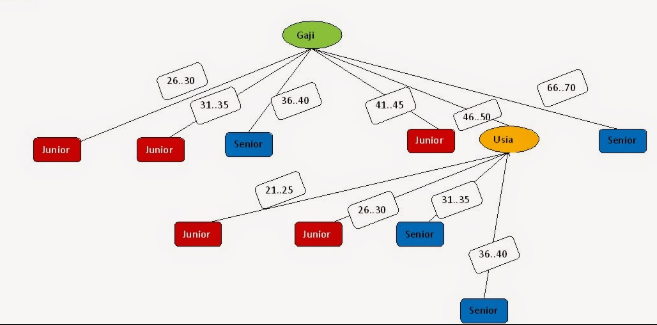
\includegraphics[width=1\textwidth]{figures/AFS/AFS1.png}}
		\caption{Random Forest.}
		\label{AFS1}
		\end{figure}

\item Cara Membaca Dataset
	

		\begin{enumerate}
			\item Buka Anaconda Navigator.
			\item Jalankan Spyder
			\item Import libraries yang dibutuhkan
			\item Masukan kode berikut untuk membaca file Data.csv.
				\begin{figure}[ht]
				\centering
				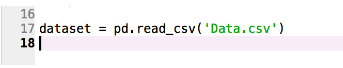
\includegraphics[scale=0.8]{figures/AFS/2.png}
				\caption{Kode membaca file.csv}
				\label{contoh}
				\end{figure}
			\item Jalankan kode tersebut, maka di windiws console akan muncul pesan :
				\begin{figure}[ht]
				\centering
				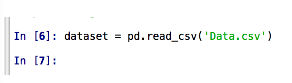
\includegraphics[scale=0.9]{figures/AFS/3.png}
				\caption{ Window Console}
				\label{contoh}
				\end{figure}
			\item Klik variable explorer, maka akan terlihat dataset yang baru ter-import.
				\begin{figure}[ht]
				\centering
				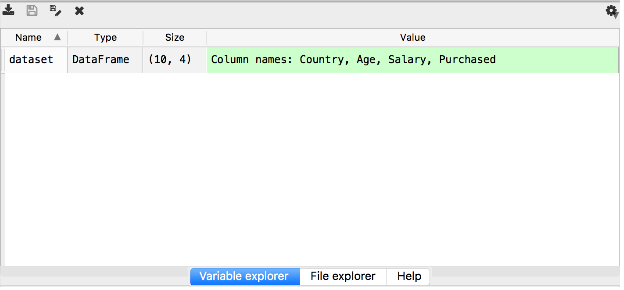
\includegraphics[scale=0.6]{figures/AFS/4.png}
				\caption{Variable Explorer}
				\label{contoh}
				\end{figure}
			\item Kemudian double klik pada dataset cell, maka akan muncul pop-up windows seperti berikut: 
				\begin{figure}[ht]
				\centering
				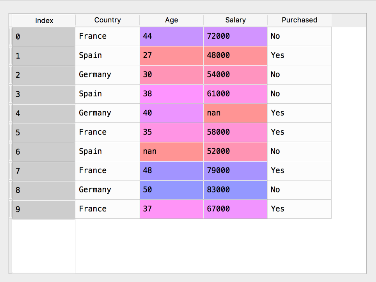
\includegraphics[scale=0.7]{figures/AFS/5.png}
				\caption{ Dataset Cell}
				\label{contoh}
				\end{figure}
			\item Seperti yang terlihat pada gambar tersebut dataset ini memiliki Kolom Country, Age, dan Salary sebagai 		   				independent variable-nya dan kolom Purchased sebagai dependent variable-nya.			
		\end{enumerate}
	

\item Cross Validation \par
Cross validation adalah metode statistik yang digunakan untuk memperkirakan keterampilan model pembelajaran mesin. Ini biasanya digunakan dalam pembelajaran mesin yang diterapkan untuk membandingkan dan memilih model untuk masalah pemodelan prediktif yang diberikan karena mudah dipahami, mudah diimplementasikan, dan menghasilkan estimasi keterampilan yang umumnya memiliki bias lebih rendah daripada metode lainnya.

\item Arti Score 44\% Pada Random Forest, 27\% Pada Decision Tree dan 29\% Dari SVM \par
\begin{enumerate}
\item Arti Score 44\% \par
Pada Random Forest, Score tersebut merupakan hasil dari akurasi.
\item Arti Score 27\% \par
Pada decission tree adalah presentasi hasil dari perhitungan dataset.
\item Arti Score 29\% Pada SVM \par
merupakan hasil pendekatan jaringan saraf. Jaringan saraf sendiri merupakan komponen jaringan utama dari sistem saraf. Sistem tersebut mengatur dan mengontrol fungsi tubuh dan aktivitas dan terdiri dari dua bagian:  (SSP) yang terdiri dari otak dan sumsum tulang belakang, dan percabangan saraf perifer dari sistem saraf tepi (SST) yang terdapat dalam pengolahan dataset terkait. 
\end{enumerate}

\begin {enumerate}
\item Confusion Matrix Dan Ilustrasinya
\end{enumerate}

\begin{enumerate}
\item Perhitungan confusion matrix adalah sebagai berikut, akan saya beri contoh sederhana yaitu pengambilan keputusan untuk mendapatkan bantuan beasiswa. Saya menggunakan dua atribut, yaitu rekening listrik dan gaji. Ini adalah pohon keputusannya:
 
\begin{figure}[ht]
\centering
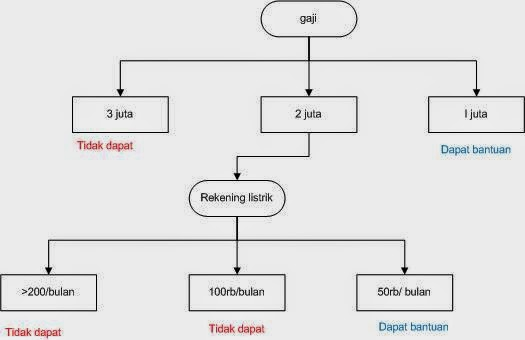
\includegraphics[scale=0.5]{figures/AFS/7.jpg}
\caption{Pohon Keputusan}
\label{contoh}
\end{figure}

\end{enumerate}


Kemudian data testingnya adalah

\begin{figure}[ht]
\centering
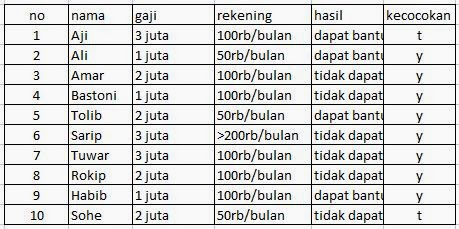
\includegraphics[scale=0.5]{figures/AFS/8.jpg}
\caption{Data Testing}
\label{contoh}
\end{figure}

Yang pertama kita lakukan yaitu mencari 4 nilai yaitu a,b,c, dan d:

 a= 5

 b= 1

 c= 1

 d= 3

Kemudian kita dapat mencari nilai Recall, Precision, accuracy dan Error Rate

 Recall =3/(1+3) = 0,75

 Precision = 3/(1+3) = 0,75

 Accuracy =(5+3)/(5+1+1+3) = 0,8

 Error Rate =(1+1)/(5+1+1+3) = 0,2

\item Jelaskan Voting Pada Random Forest Beserta Ilustrasinya 
\par Voting merupakan metode yang paling umum digunakan dalam random forest. Ketika classifier membuat keputusan, Anda dapat memanfaatkan yang terbaik keputusan umum dan rata-rata yang didefinisikan ke dalam bentuk "voting".
\par Setelah pohon terbentuk,maka akan dilakukan voting pada setiap kelas dari data sampel. Kemudian, mengkombinasikan vote dari setiap kelas kemudian diambil vote yang paling banyak.Dengan menggunakan random forest pada klasifikasi data maka, akan menghasilkan vote yang paling baik. \ref{AFS6}
		\begin{figure}[ht]
		\centerline{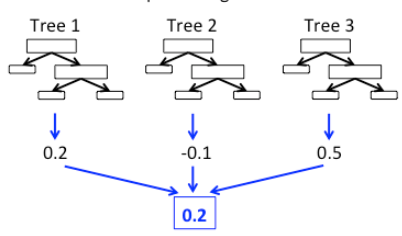
\includegraphics[width=1\textwidth]{figures/AFS/6.png}}
		\caption{Voting.}
		\label{AFS6}
		\end{figure}



\subsection{Praktek Program}
\begin{enumerate}
\item Aplikasi Sederhana Menggunakan Pandas
	\begin{figure}[ht]
	\centering
	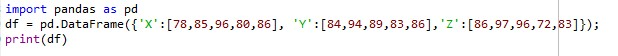
\includegraphics[scale=0.5]{figures/AFS/praktek1.jpg}
	\caption{Aplikasi Pandas}
	\label{contoh}
	\end{figure}

\end{enumerate}
	\par Penjelasan kodingan :
		\begin{enumerate}
		\item Memanggil library.
		\item Membuat variable dengan data frame.
		\item Menampilkan hasil
		\end{enumerate}
	\par Sehingga menghasilkan :
	\begin{figure}[ht]
	\centering
	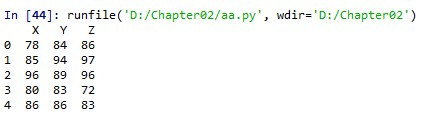
\includegraphics[scale=0.5]{figures/AFS/praktek2.jpg}
	\caption{Hasil Pandas}
	\label{contoh}
	\end{figure}
\item Aplikasi Sederhana Menggunakan Numpy
	\begin{figure}[ht]
	\centering
	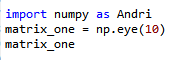
\includegraphics[scale=0.5]{figures/AFS/praktek3.png}
	\caption{Aplikasi Numpy}
	\label{contoh}
	\end{figure}
	\par Penjelasan kodingan :
		\begin{enumerate}
		\item Memanggil library numpy
		\item Membuat variable dengan value eye dengan size10
		\item Menampilkan hasil value
		\end{enumerate}
	\par Sehingga menghasilkan :
	\begin{figure}[ht]
	\centering
	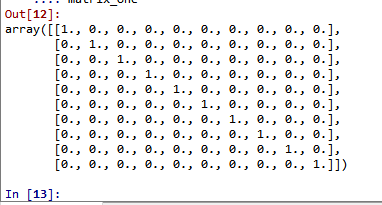
\includegraphics[scale=0.5]{figures/AFS/praktek4.png}
	\caption{Hasil Numpy}
	\label{contoh}
	\end{figure}
\item Aplikasi Sederhana Menggunakan Matplotlib
	\begin{figure}[ht]
	\centering
	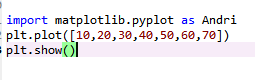
\includegraphics[scale=0.5]{figures/AFS/praktek5.png}
	\caption{Aplikasi Matplotlib}
	\label{contoh}
	\end{figure}
	\par Penjelasan kodingan :
		\begin{enumerate}
		\item Memanggil library matplotlib.pyplot
		\item Membuat variable yang berisi 10,20,30,40,50,60,70
		\item Membuat garis koordinat
		\item Menampilkan hasil plt
		\end{enumerate}
	\par Sehingga menghasilkan :
	\begin{figure}[ht]
	\centering
	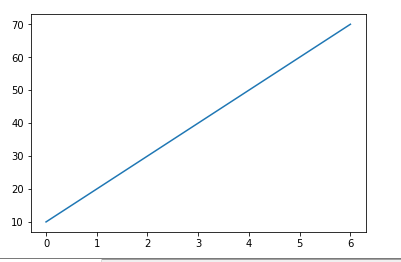
\includegraphics[scale=0.5]{figures/AFS/praktek6.png}
	\caption{Hasil Matplotlib}
	\label{contoh}
	\end{figure}
\par
\par
\item Program Klasifikasi Random Forest :
\begin{itemize}
\item Code Random Forest 1 :
\par
\begin{figure}[ht]
\centering
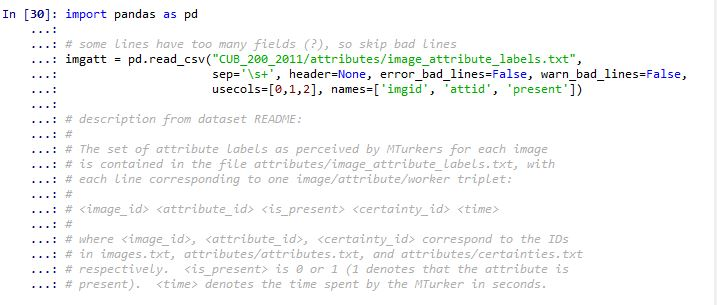
\includegraphics[scale=0.7]{figures/AFS/4a.jpg}
\caption{Gambar1}
\label{contoh}
\end{figure}
\par
\end{itemize}

\begin{itemize}
\item Penjelasan : Membaca dataset. Codingan di atas menghasilkan variabel baru yaitu imgatt. Terdapat 3 kolom dan 3677856 baris data.
\par 
\par
\end{itemize}
\item Code Random Forest 2 :
\par
\begin{figure}[ht]
\centering
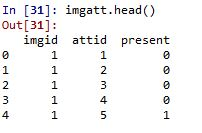
\includegraphics[scale=0.7]{figures/AFS/4b.jpg}
\caption{Gambar2}
\label{contoh}
\end{figure}
\par
\begin{itemize}
\item Penjelasan : Codingan di atas berfungsi untuk melihat sebagian data awal dari dataset. Hasilnya terdapat pada gambar di atas setelah di eksekusi.
\par
\par
\end{itemize}
\item Code Random Forest 3 :
\par
\begin{figure}[ht]
\centering
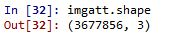
\includegraphics[scale=0.7]{figures/AFS/4c.jpg}
\caption{Gambar3}
\label{contoh}
\end{figure}
\par
\begin{itemize}
\item Penjelasan : Codingan di atas merupakan tampilan untuk menampilkan hasil dari dataset yang telah di run atau di eksekusi. Dimana pada gambar di atas 3677856 merupakan baris dan 3 adalah kolom.
\par
\par
\end{itemize}
\item Code Random Forest 4 :
\par
\begin{figure}[ht]
\centering
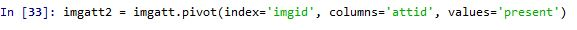
\includegraphics[scale=0.7]{figures/AFS/4d.jpg}
\caption{Gambar 4}
\label{contoh}
\end{figure}
\par
\begin{itemize}
\item Penjelasan : Pada gambar di atas menmapilkan hasil dari variabel imgatt2. Dimana index nya 'imgid', kolom berisi 'attid' dan values atau nilainya berisi 'present'.
\par
\par
\end{itemize}
\item Code Random Forest 5 :
\par
\begin{figure}[ht]
\centering
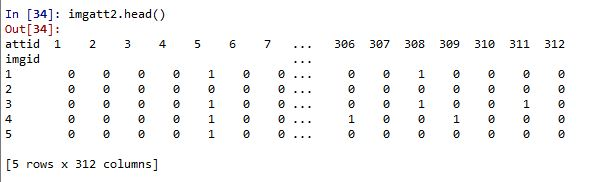
\includegraphics[scale=0.7]{figures/AFS/4e.jpg}
\caption{Gambar 5}
\label{contoh}
\end{figure}
\par
\begin{itemize}
\item Penjelasan : Pada gambar di atas menmapilkan hasil dari variabel imgatt2.head. Dimana dataset nya ada 5 baris dan 312 kolom.
\par
\par
\end{itemize}
\item Code Random Forest 6 :
\par
\begin{figure}[ht]
\centering
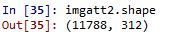
\includegraphics[scale=0.7]{figures/AFS/4f.jpg}
\caption{Gambar 6}
\label{contoh}
\end{figure}
\par
\begin{itemize}
\item Penjelasan : Pada gambar di atas menampilkan jumlah dari baris dan kolom dari variabel imgatt2. Dimana 11788 adalah baris dan 312 adalah kolom.
\par
\par
\end{itemize}
\item Code Random Forest 7 :
\par
\begin{figure}[ht]
\centering
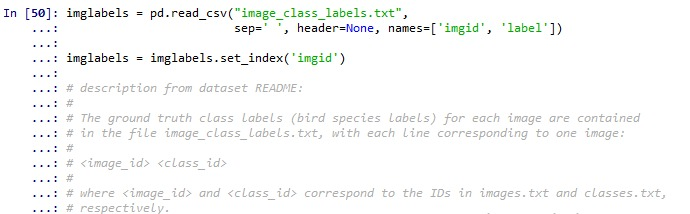
\includegraphics[scale=0.7]{figures/AFS/4g.jpeg}
\caption{Gambar 7}
\label{contoh}
\end{figure}
\par
\begin{itemize}
\item Penjelasan : Pada gambar di atas menunjukkan load dari  jawabannya yang berisi " apakah burung tersebut ( subjek pada dataset ) termasuk dalam spesies yang mana ?. Kolom yang digunakan adalah imgid dan label, kemudian melakukan pivot yang mana imgid menjadi index yang artinya unik sehubungan dengan dataset yang telah dieksekusi.
\par
\par
\end{itemize}
\item Code Random Forest 8 :
\par
\begin{figure}[ht]
\centering
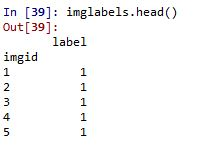
\includegraphics[scale=0.2]{figures/AFS/4h.jpg}
\caption{Gambar 8}
\label{contoh}
\end{figure}
\par
\begin{itemize}
\item Penjelasan : Pada gambar di atas menunjukkan hasil dari variabel imglabels. Dimana menampilkan dataset dari imgid dan label. Dan dapat dilihat hasilnya dari gambar di atas.
\par
\par
\end{itemize}
\item Code Random Forest 9 :
\par
\begin{figure}[ht]
\centering
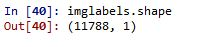
\includegraphics[scale=0.7]{figures/AFS/4i.jpg}
\caption{Gambar 9}
\label{contoh}
\end{figure}
\par
\begin{itemize}
\item Penjelasan : Pada gambar di atas menunjukkan jumlah baris dan kolom dari variabel imglabels. Dimana hasil dari kodingan tersebut dapat dilihat setelah di run. 
\par
\par
\end{itemize}
\item Code Random Forest 10 :
\par
\begin{figure}[ht]
\centering
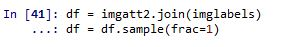
\includegraphics[scale=0.7]{figures/AFS/4j.jpg}
\caption{Gambar 10}
\label{contoh}
\end{figure}
\par
\begin{itemize}
\item Penjelasan : Pada gambar diatas dikarenakan isinya sama, maka bisa melakukan join antara dua data yang diesekusi ( yaitu ada imgatt2 dan imglabels ), sehingga pada hasilnya akan didapatkan data ciri dan data jawaban atau labelnya sehingga bisa dikategorikan/dikelompokkan sebagai supervised learning. Jadi perintah untuk menggabungkan kedua data, kemudian dilakukan pemisahan antara data set untuk training dan test pada dataset yang dieksekusi.
\par
\par
\end{itemize}
\item Code Random Forest 11 :
\par
\begin{figure}[ht]
\centering
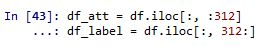
\includegraphics[scale=0.7]{figures/AFS/4k.jpg}
\caption{Gambar 11}
\label{contoh}
\end{figure}
\par
\begin{itemize}
\item Penjelasan :Pada gambar di atas menghasilkan pemisahan dan pemilihan tabel ( memisahkan dan memilih tabel ). 
\par
\par
\end{itemize}
\item Code Random Forest 12 :
\par
\begin{figure}[ht]
\centering
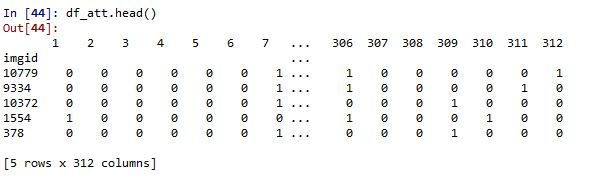
\includegraphics[scale=0.7]{figures/AFS/4l.jpg}
\caption{Gambar 12}
\label{contoh}
\end{figure}
\par
\begin{itemize}
\item Penjelasan : Pada gambar di atas menunjukkan hasil dari variabel dtatthead. Dimana data nya dapat dilihat pada gambar diatas. Dan dataset nya terdiri dari 5 baris dan 312 kolom.
\par
\par
\end{itemize}
\item Code Random Forest 13 :
\par
\begin{figure}[ht]
\centering
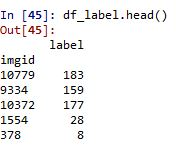
\includegraphics[scale=0.7]{figures/AFS/4m.jpg}
\caption{Gambar 13}
\label{contoh}
\end{figure}
\par
\begin{itemize}
\item Penjelasan : Pada gambar di atas menunjukkan hasil dari variabel dflabel.head. Dimana berisikan data dari imgid dan label. Dan hasilnya dapat dilihat pada gambar di atas.
\par
\par
\end{itemize}
\item Code Random Forest 14 :
\par
\begin{figure}[ht]
\centering
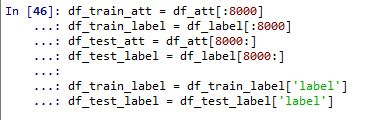
\includegraphics[scale=0.7]{figures/AFS/4n.jpg}
\caption{Gambar 14}
\label{contoh}
\end{figure}
\par
\begin{itemize}
\item Penjelasan : Pada gambar di atas merupakan pembagian dari data training dan dataset
\par
\par
\end{itemize}
\item Code Random Forest 15 :
\par
\begin{figure}[ht] 
\centering
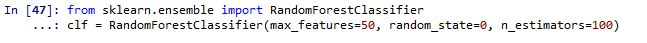
\includegraphics[scale=0.7]{figures/AFS/4o.jpg}
\caption{Gambar 15}
\label{contoh}
\end{figure}
\par
\begin{itemize} 
\item Penjelasan : Pada gambar di atas merupakan pemanggilan kelas RandomForestClassifier. max features yang diartikan berapa banyak kolom pada setiap tree.
\par
\par
\end{itemize}
\item Code Random Forest 16 :
\par
\begin{figure}[ht]
\centering
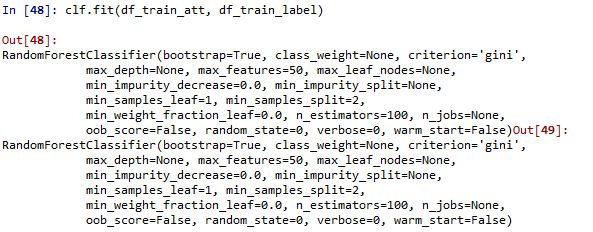
\includegraphics[scale=0.7]{figures/AFS/4p.jpg}
\caption{Gambar 16}
\label{contoh}
\end{figure}
\par
\begin{itemize}
\item Penjelasan : Pada gambar di atas merupaka perintah untuk melakukan fit untuk membangun random forest yang sudah ditentukan dengan maksimum fitur sebanyak 50.
\par
\par
\end{itemize}
\item Code Random Forest 17 :
\par
\begin{figure}[ht]
\centering
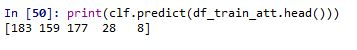
\includegraphics[scale=0.7]{figures/AFS/4q.jpg}
\caption{Gambar 17}
\label{contoh}
\end{figure}
\par
\begin{itemize}
\item Penjelasan : Pada gambar di atas menunjukkan hasil dari cetakan variabel dftrainatt.head.
\par
\par
\end{itemize}
\item Code Random Forest 18 :
\par
\begin{figure}[ht]
\centering
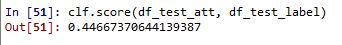
\includegraphics[scale=0.7]{figures/AFS/4r.jpg}
\caption{Gambar 18}
\label{contoh}
\end{figure}
\par
\begin{itemize}
\item Penjelasan : Pada gambar di atas merupakan hasil dari variabel dftestatt da dftsetlabel. Dimana hasilnya dapat dilihat dari pada gambar di atas
\par
\par
\end{itemize}

\item Program Klasifikasi Confusion Matrix
	\begin{itemize}
		\item Setelah melakukan random forest kemudian dipetakan ke dalam confusion matrix.
			\begin{figure}[ht]
			\centering
			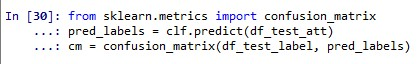
\includegraphics[scale=0.5]{figures/AFS/abc1.jpg}
			\caption{Memetakan ke confusion matrix}
			\label{contoh}
			\end{figure}
		\item Lalu melihat hasilnya.
			\begin{figure}[ht]
			\centering
			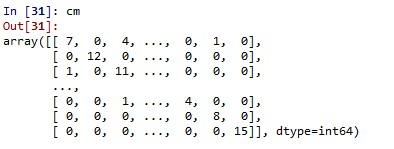
\includegraphics[scale=0.5]{figures/AFS/abc2.jpg}
			\caption{Melihat hasil}
			\label{contoh}
			\end{figure}
		\item Kemudian dilakukan perintah plot.
			\begin{figure}[ht]
			\centering
			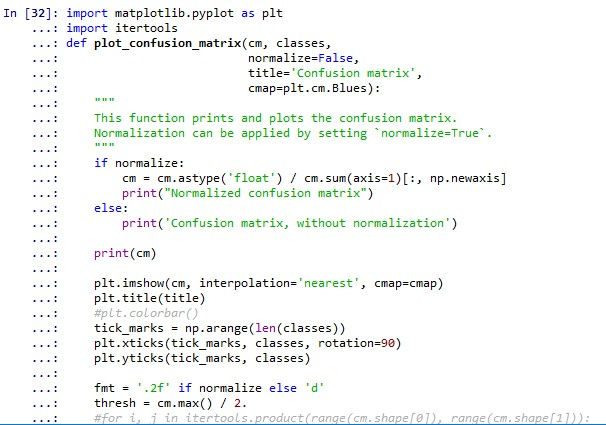
\includegraphics[scale=0.5]{figures/AFS/abc3.jpg}
			\caption{Melakukan Plot}
			\label{contoh}
			\end{figure}
		\item Selanjutnya nama data akan di set agar plot sumbunya sesuai.
			\begin{figure}[ht]
			\centering
			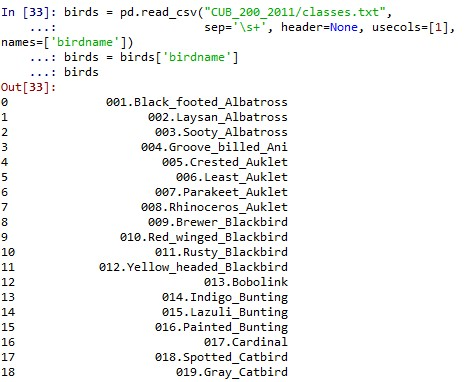
\includegraphics[scale=0.5]{figures/AFS/abc4.jpg}
			\caption{Plotting nama data}
			\label{contoh}
			\end{figure}
		\item Setelah label berubah, maka dilakukan perintah plot.
		\begin{figure}[ht]
			\centering
			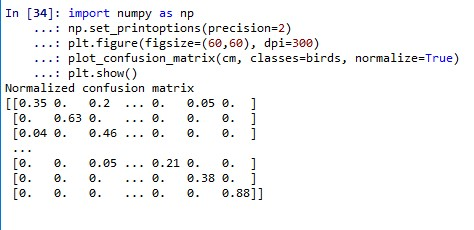
\includegraphics[scale=0.5]{figures/AFS/abc5.jpg}
			\caption{Melakukan perintah plot}
			\label{contoh}
			\end{figure}
	\end{itemize}
\par
\par
\item Program Klasifikasi SVM dan Decision Tree Beserta Penjelasan Keluarannya :
\begin{itemize}
\item Code SVM :
\par
\begin{figure}[ht]
\centering
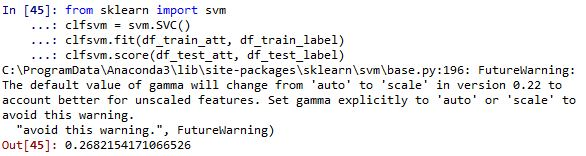
\includegraphics[scale=0.7]{figures/AFS/t2.jpg}
\caption{SVM}
\label{contoh}
\end{figure}
\par
\end{itemize}

\begin{itemize}
\item Penjelasan : Pada gambar di atas cara untuk mencoba klasikasi dengan SVM dengan dataset yang sama.
\par 
\par
\end{itemize}
\item Code Decision Tree :
\par
\begin{figure}[ht]
\centering
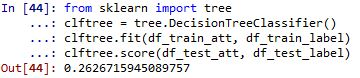
\includegraphics[scale=0.7]{figures/AFS/t1.jpg}
\caption{Decission Tree}
\label{contoh}
\end{figure}
\par
\begin{itemize}
\item Penjelasan : Pada gambar di atas merupakan cara untuk mencoba klasikasi dengan decission tree dengan dataset yang sama.
\par
\par

\end{itemize}


\item Program Cross Validation
	\begin{itemize}
		\item Melakukan pengecekan cross validation untuk random forest.
			\begin{figure}[ht]
			\centering
			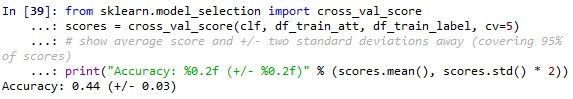
\includegraphics[scale=0.5]{figures/AFS/fajar1.jpg}
			\caption{Pengecekan cross validation random forest}
			\label{contoh}
			\end{figure}
		\item Melakukan pengecekan cross validation untuk decission tree.
			\begin{figure}[ht]
			\centering
			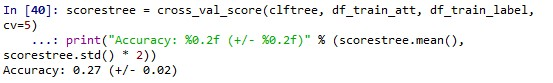
\includegraphics[scale=0.5]{figures/AFS/fajar2.jpg}
			\caption{Pengecekan cross validation decision tree}
			\label{contoh}
			\end{figure}
		\item Melakukan pengecekan cross validation untuk SVM.
	\end{itemize}

\item Program Pengamatan Komponen Informasi
	\begin{itemize}
		\item Melakukan pengamatan komponen informasi untuk menetahui berapa banyak tree yang dibuat, atribut yang dipakai, dan informasi lainnya.
			\begin{figure}[ht]
			\centering
			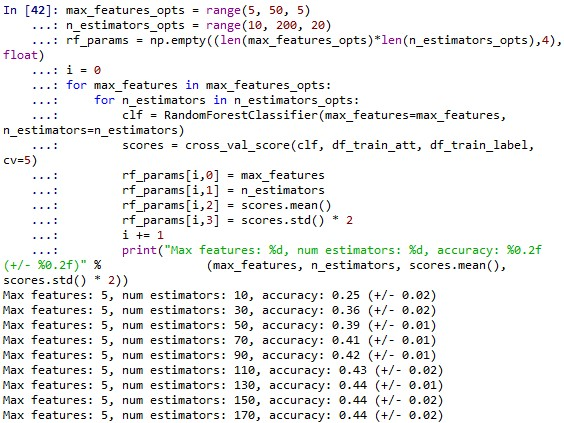
\includegraphics[scale=0.5]{figures/AFS/sunandhar1.jpg}
			\caption{Pengamatan Komponen}
			\label{contoh}
			\end{figure}
		\item Melakukan plot informasi agar bisa dibaca.
			\begin{figure}[ht]
			\centering
			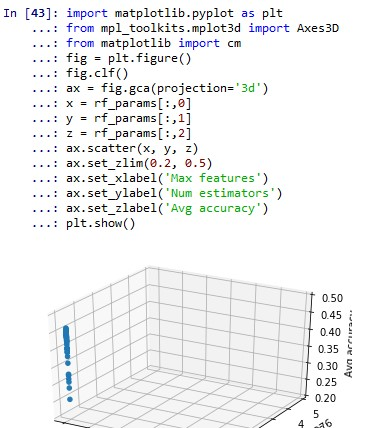
\includegraphics[scale=0.5]{figures/AFS/sunandhar2.jpg}
			\caption{Plot informasi}
			\label{contoh}
			\end{figure}
	\end{itemize}
\end{enumerate}

\par
\par
\subsection{Penanganan Eror}
Penyelesaian Tugas Harian  ( Penanganan Error )
\begin{enumerate}
\item Menyelesaikan dan Membahas Penanganan Error :
\begin{itemize}
\item Skrinsut Error

\begin{figure}[ht]
\centering
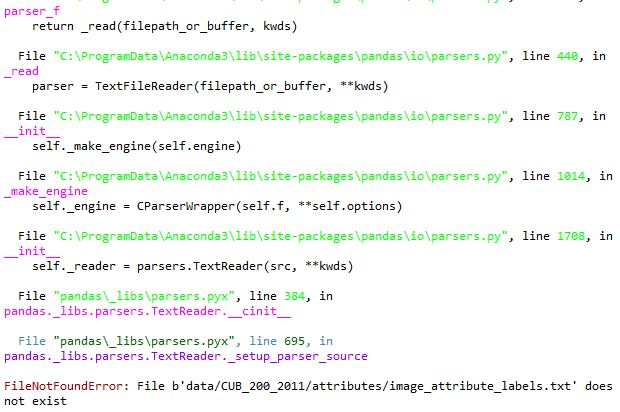
\includegraphics[scale=0.7]{figures/AFS/Error.jpg}
\caption{Error}
\label{contoh}
\end{figure}
\end{itemize}

\begin{itemize}
\item Kode Error: file b'data/CUB 200 2011/attributes/image attributes labels.txt'
\par 
\item Solusi Pemecahan Error : Hapus Direktori data pada kode pastikan satu folder.
\par 
\par
\end{itemize}
\end{enumerate}
